% Latex Template for arbitrary format proposals
% 2016-12-2
% S. Rodney 
%----------------------------------------------------------------------%

\documentclass[12pt]{article}
\usepackage[top=0.8in, bottom=0.8in, left=0.8in, right=0.8in]{geometry}
%\usepackage{times}
%\usepackage{color}
\usepackage{setspace}
%\usepackage{charter}
\usepackage{graphicx}
\usepackage{minibox}
\usepackage{fancyhdr}
\usepackage{subcaption}
\usepackage[font=scriptsize]{caption}
\usepackage{amssymb}
\usepackage{wrapfig}

%%%%%%%%%%%%%%%%%%%%%%%%%%%%%%%%%%%%%%%%%%%%%%%%%%%
% PDF mode settings : Auto-select eps or pdf figures 
% based  on the compiler used (i.e. latex vs pdflatex)
%%%%%%%%%%%%%%%%%%%%%%%%%%%%%%%%%%%%%%%%%%%%%%%%%%%
\ifx\pdfoutput\undefined
  \pdffalse
  \DeclareGraphicsExtensions{.eps,.ps}
\else
  \ifnum\pdfoutput=1
    % \pdftrue
    \DeclareGraphicsExtensions{.pdf,.png,.jpg}
  \else
    % \pdffalse
    \DeclareGraphicsExtensions{.eps,.ps}
  \fi
\fi



\begin{document}
\thispagestyle{empty}
\onehalfspace
  
%
% USC Logo, centered
\begin{center}

\includegraphics[width=2.8in,draft=False]{USC_Standard_CMYK}%}}
\end{center}
\bigskip

\noindent {\bf Proposal to the South Carolina Space Grant Consortium\\}
\noindent {\bf NASA EPSCoR Research Grant Program (\$25k)}
\bigskip

\noindent {\bf PI: Steven A. Rodney}\\
Department of Physics \& Astronomy\\
University of South Carolina\\
712 Main Street,  Jones PSC 404\\
Columbia, SC  29208\\
803-777-2599  \\  
srodney@sc.edu
\bigskip

\noindent {\bf Project Title:}\\
Rare and Peculiar Stellar Explosions with the Next Generation of Space Telescopes
\bigskip

\noindent {\bf NASA Alignment:}
\begin{itemize}
\item Science Mission Directorate (SMD) - Astrophysics Division
\end{itemize}
\bigskip

\noindent {\bf Related NASA Centers:}
\begin{itemize}
\item Space Telescope Science Institute (Baltimore, MD)
\item NASA Goddard Space Flight Center (Greenbelt, MD)
\item Infrared Processing and Analysis Center (Pasadena, CA)
\end{itemize}


%\pagebreak
\thispagestyle{fancy}
% Leave Left and Right Header empty.
\lhead{}
\rhead{}
\renewcommand{\headrulewidth}{1pt}
\renewcommand{\footrulewidth}{0pt}
\newcommand{\packageName}{\textit{SNTD}}
\fancyfoot[C]{}

\pagestyle{fancy}
\lhead{\bf SC NASA EPSCoR GRA    \  $\|$}
\rhead{\bf Justin D. Roberts-Pierel, University of South Carolina}

Observing and understanding gravitationally lensed objects is a new
and exciting field of study. The first example of a strongly lensed
supernova (SN) resolved into multiple images was SN ``Refsdal'' in
2014 (Figure 1; \citet{Kelly:2015a}). Subsequent work was done to
classify Refsdal, as well as to measure time delays and magnification
ratios \citep{Kelly:2016,Rodney:2016}. To date, there is no optimally
designed software package to analyze correlated data sets from
multiply imaged lensed SNe and simultaneously determine SN class, time
delays, and magnification ratios. The lack of a standard resource
leaves researchers to write and implement their own ad hoc programs,
which increases uncertainty and decreases efficiency. It's clear that
an optimized software package with the ability to analyze a light
curve for these and other parameters would be extremely valuable to a
wide range of research using current and next generation telescopes.

\begin{figure}[h]
\centering
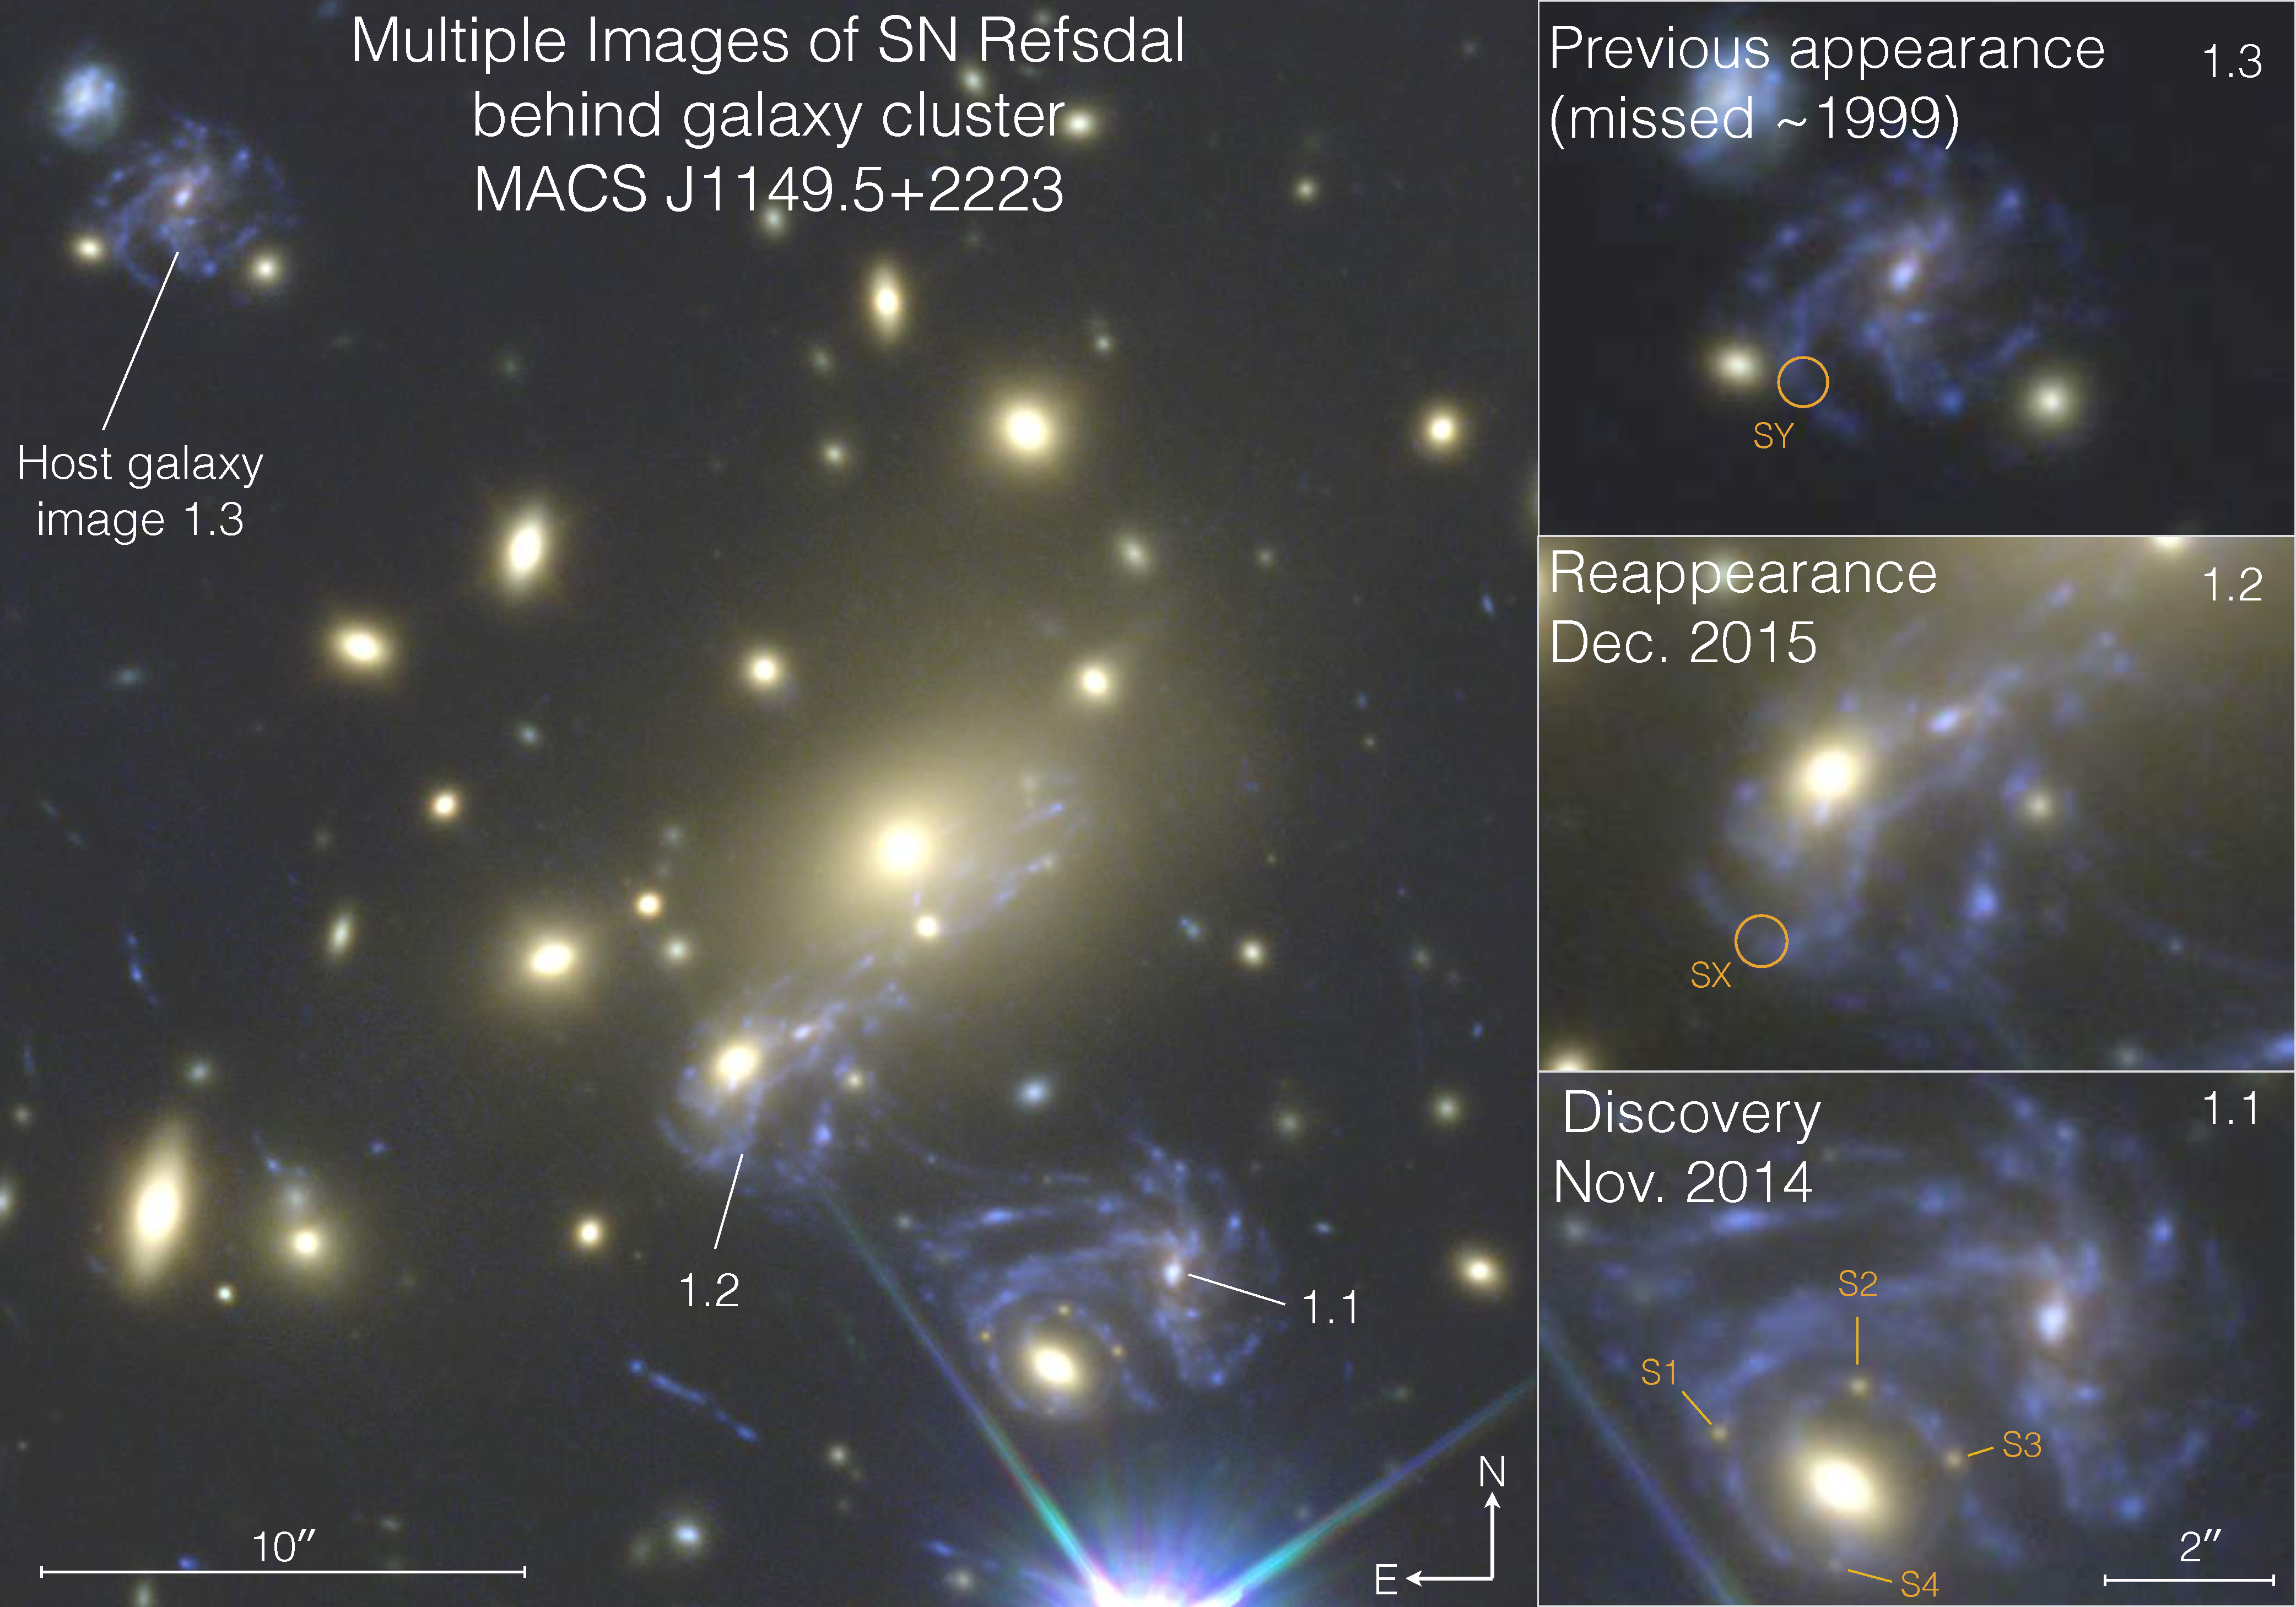
\includegraphics[width=0.9\textwidth]{refsdal_rodney.pdf}
\caption{
MACS J1149.6+2223 field, showing the positions of the three primary
images of the SN Refsdal host galaxy (labeled 1.1, 1.2, and 1.3). SN
Refsdal appears as four point sources in an Einstein Cross
configuration in the southeast spiral arm of image 1.1 (2)}
\end{figure}


The purpose of this work is to produce an open-source software
package called Supernova Time Delays ($\packageName$) that will
address the SN modeling needs of the research community and lead to a
first-author publication that furthers our understanding of lensed
SNe. There are currently two software packages, written in Python,
which are relevant to this product: Python Curve Shifting (PyCS), and
Supernova Cosmology (SNCosmo). There will be four components to this
research: 1) Integrate SNCosmo and PyCS, giving researchers a tool
that can model SN light curve data with the tools present in either
software package; 2) Extend and optimize lensing and microlensing
algorithm present in PyCS for SNe; 3) Simulate a large number of SN
light curves using SNCosmo and test the ability of $\packageName$ to
determine SN parameters; and 4) Explore the abilities of
$\packageName$ in analyzing POP III SNe using modeled light curves in
anticipation of JWST and WFIRST observations.

%\begin{figure}[h]
%\centering
%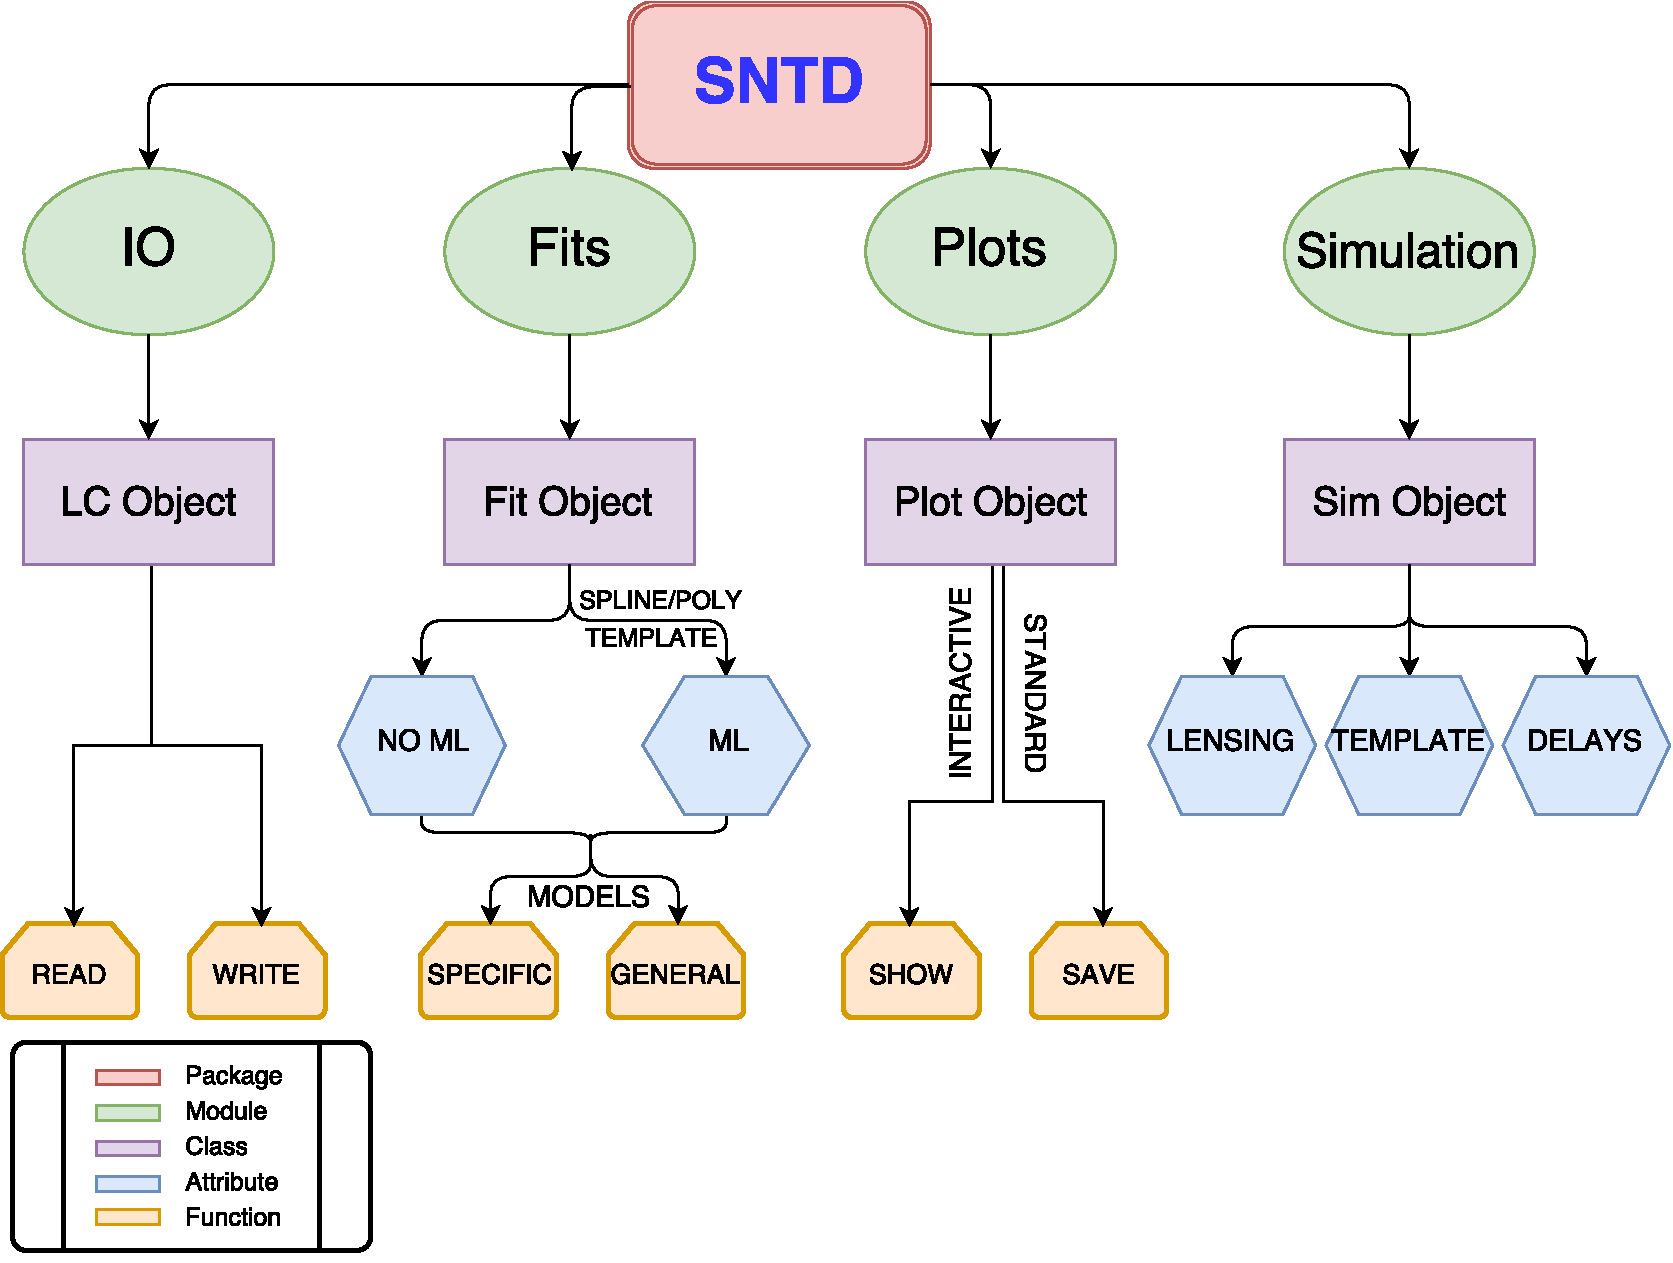
\includegraphics[scale=.38]{gra_2017_Flow2.pdf}
%\caption{A visual representation of the capabilities of SNTD. The python package will have a simple framework in which each module creates a respective object, which can then be edited by the user. This structure is extremely organized, computationally efficient, and user-friendly.}
%\end{figure}


While PyCS currently uses flexible functions to account for
microlensing of quasars caused by transverse motion of stars in the
lensing galaxy, there is a second form of microlensing unique to
lensed SNe. The expanding photosphere of a SN interacts with
intervening matter, causing microlensing effects described by Dobler
and Keeton 2006a that can exhibit magnitude fluctuations of $\sim$0.2
to $>$0.5 on timescales of weeks to months. This proposed work has
already integrated the flexible function method (Figure 2), and will
seek to include both types of microlensing effects to increase the
precision of time delay measurements. No software package currently
exists with this capability, therefore the algorithm will be developed
following the methodology of Dobler and Keeton 2006a. In general,
$\packageName$ will be much more likely to correctly identify SN
microlensing effects and produce simpler time delay measurements
because, unlike for quasars, researchers already have a robust set of
intrinsic light curve shapes to describe a range of different SN
classes that will allow for physically motivated, less flexible
models. By allowing certain constraints to float as free parameters,
these models will also produce best-fit synthetic light curves, from
which time delay, magnifications, SN class, and redshift can be
derived. By simulating large numbers of SNe with these synthetic light
curves, we will be able to quantify the accuracy and efficiency of the
software.


%{\setlength{\parindent}{.5cm}

%}
%\begin{figure}[h]
%\centering
%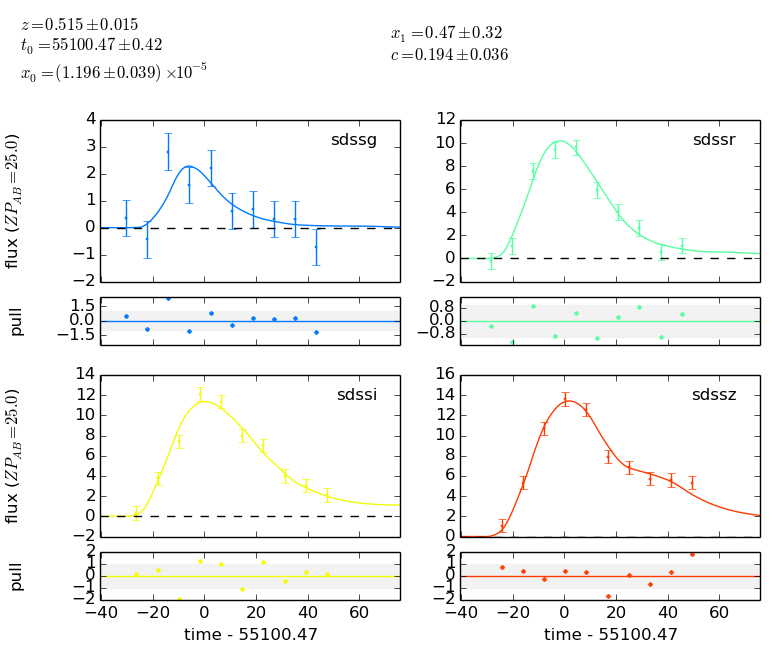
\includegraphics[scale=.4]{sncosmo.png}
%\caption{
%In addition to spline fitting (Figure 2), $\packageName$ is able to
%fit model templates to SN light curve data to measure various
%properties. In future work, the Dobler and Keeton 2006a methodology
%will be used to extract microlensing effects by identifying
%perturbations from these templates.}
%\end{figure}


 The era of JWST will yield a drastic increase SN observations at
z$<$5 (4), and WFIRST will arrive shortly thereafter in the mid
2020s. In addition, recent simulations of PI SN light curves indicate
that various solar mass PI and POP III Type IIn SNe will be visible to
both JWST (z$>$30 and z$\sim$15 respectively) and WFIRST (z$\sim$20
and z$\sim$5 respectively) (5). Whether it is a follow-up observation
of a ground based detection, or a discovery made by one of these space
telescopes, having flexible software in place to analyze any SN light
curve will be essential to SN cosmologists. We expect this research to
yield multiple publications about the methodology of the software
itself and the simulation results for low and high redshift SNe, as
well as advancements in our understanding of lensed SNe resulting from
the use of $\packageName$. There are also plans to use this package
for follow-up measurements of SN Refsdal and the PTF Type Ia SN
parameters, including the previously ignored microlensing
effects. $\packageName$ will be written in Python, a free and
open-source programming language, and distributed to SN researchers
with extensive documentation including descriptive tutorials. This
combination will make $\packageName$ a free, widely accessible, and
invaluable tool in the SN research community.  
\begin{figure}[h]

\centering
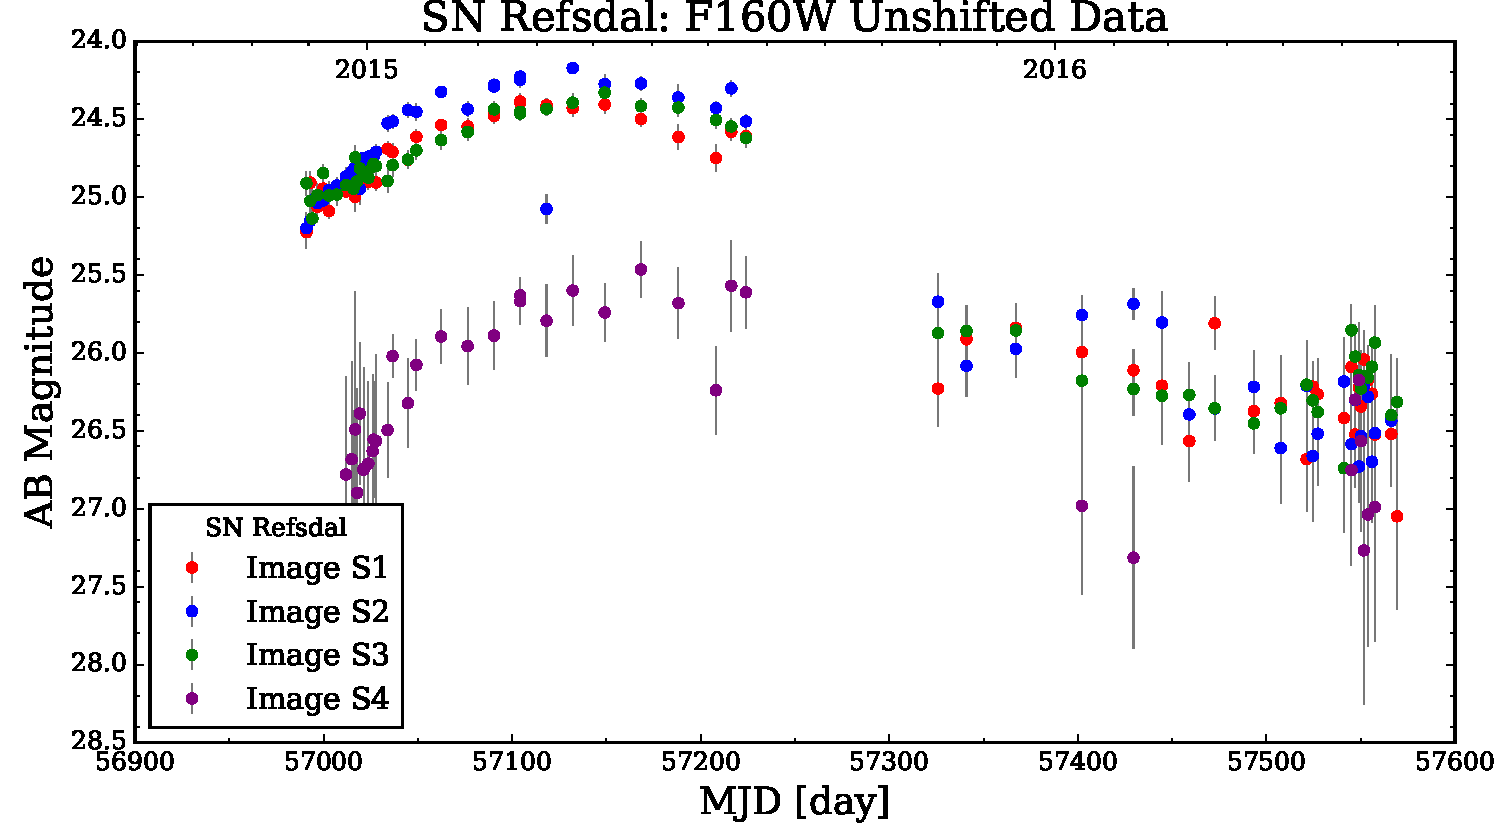
\includegraphics[width=.78\textwidth]{points_plot_2017.pdf}
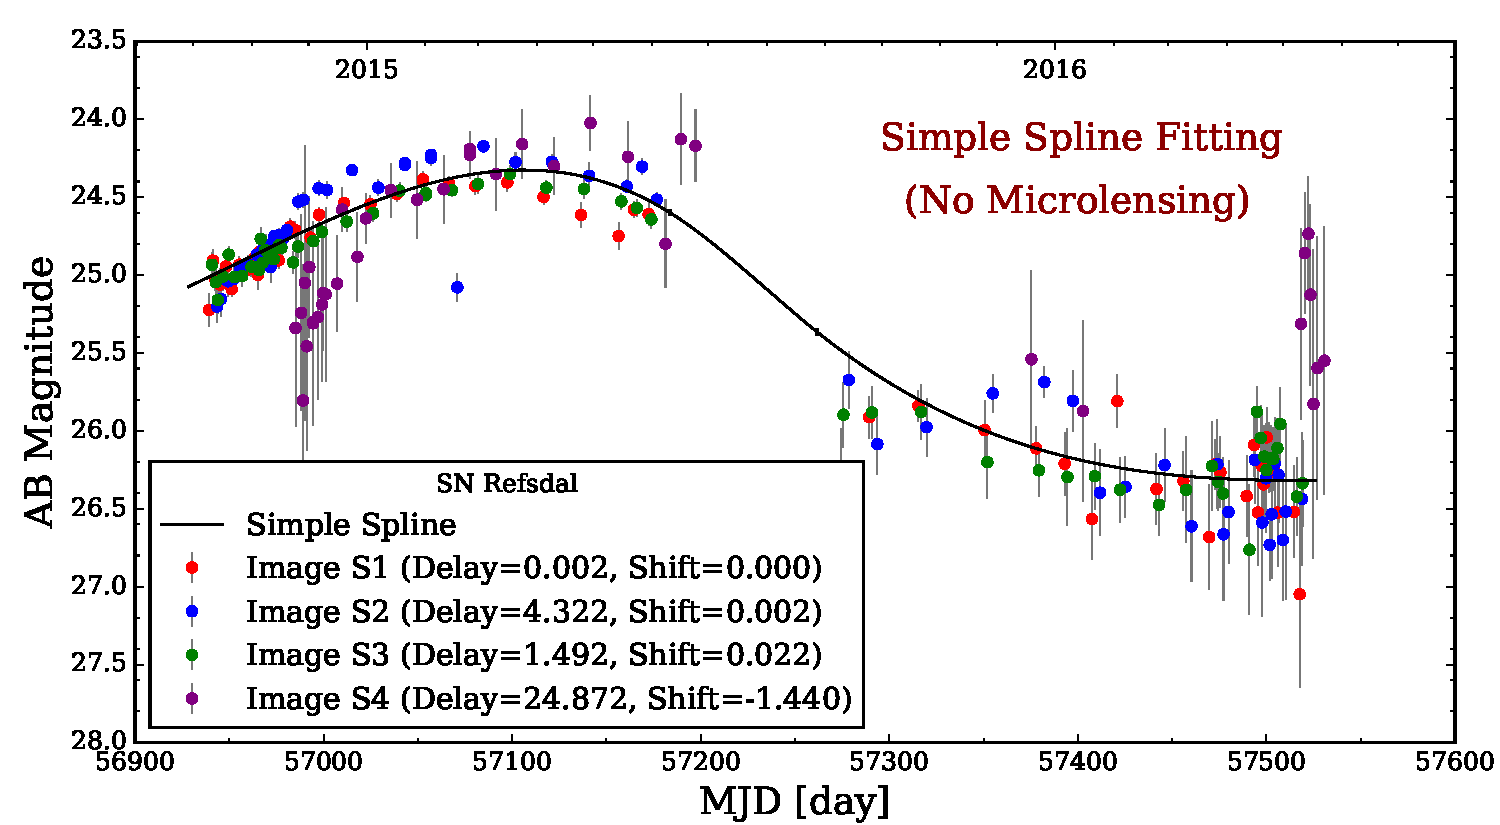
\includegraphics[width=.78\textwidth]{refs_plot_2017.pdf}
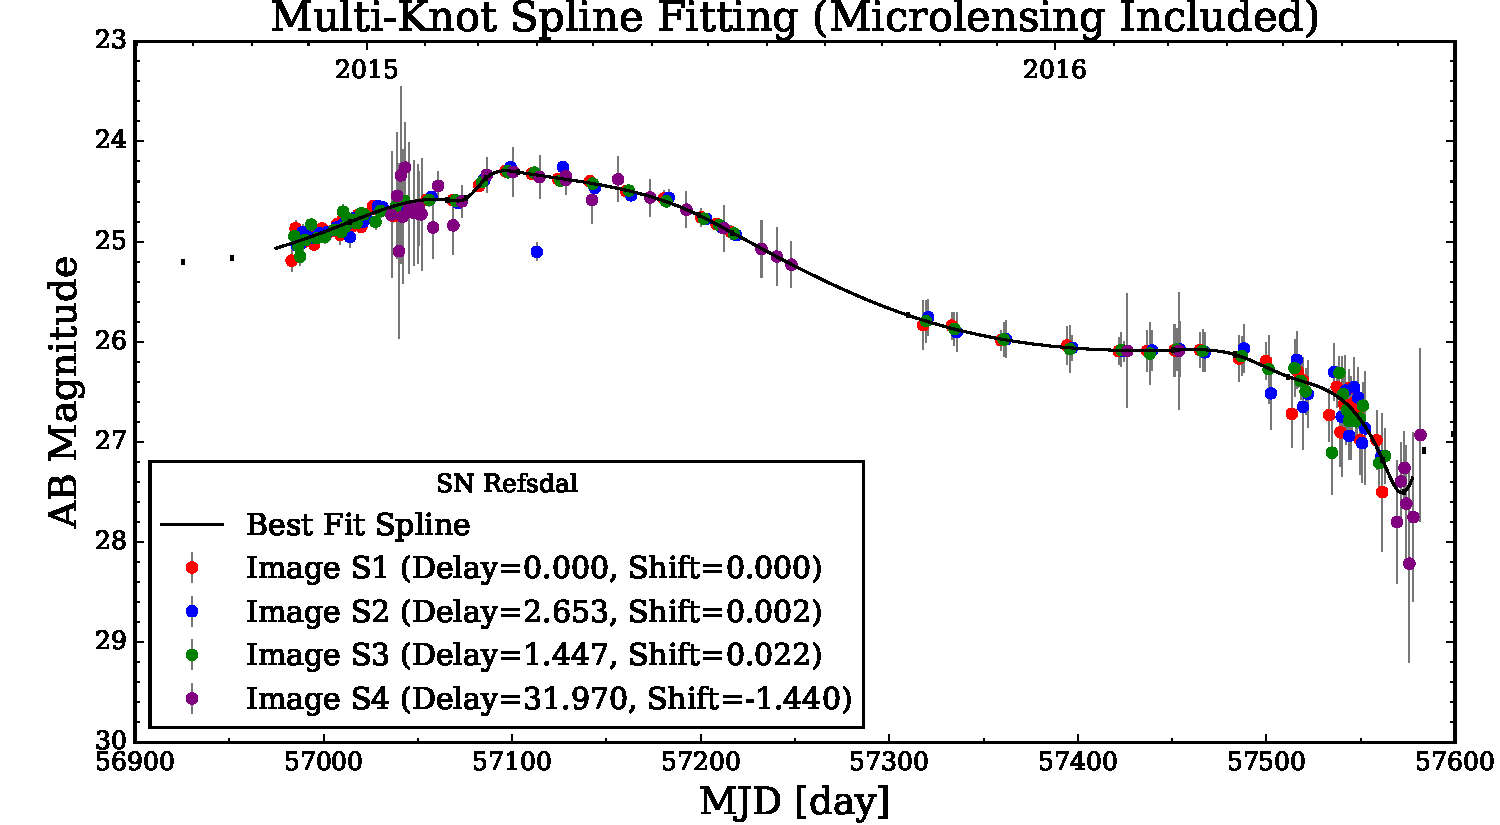
\includegraphics[width=.78\textwidth]{spline_plot_2017.pdf}
\caption{(Top) Colorized are the F160W data representing the four images of SN
Refsdal (Figure 1), with no lensing or time shifts. (Middle) Method of
fitting the SN Refsdal light curves from Rodney et al. 2016 (Bottom)
Preliminary results from $\packageName$ using a multi-knot spline to
fit the data, with lensing and time delays considered. }
\end{figure}

\pagebreak
\bibliographystyle{apjbrief}

\bibliography{bibdesk}

%\


%1. Kelly, Patrick L, Steven A Rodney, Tommaso Treu, Ryan J Foley,
%Gabriel Brammer, Kasper B Schmidt, Adi Zitrin, et
%al. 2015. ``Multiple Images of a Highly Magnified Supernova Formed by
%an Early-Type Cluster Galaxy Lens.'' Science 347 (6226):
%1123-26. doi:10.1126/science.aaa3350.

%\

%2. Rodney, S. A., L.G. Strolger, P. L. Kelly, M. Bradac, G. Brammer,
%A. V. Filippenko, R. J. Foley, et al. 2016. ``SN Refsdal: Photometry
%and Time Delay Measurements of the First Einstein Cross Supernova''
%The Astrophysical Journal 820 (1):
%50. doi:10.3847/0004-637X/820/1/50.

%\

%3. Dobler, Gregory, and Charles R Keeton. 2006. ``Microlensing of
%Lensed Supernovae.'' Astrophysical Journal.

%\

%4. Mesinger, Andrei, and Benjamin D Johnson. 2006. ``The Redshift
%Distribution of Distant Supernovae and Its Use in Probing
%Reionization'', 80-90.

%\

%5. Magg, Mattis, Tilman Hartwig, Simon C O Glover, Ralf S Klessen,
%and J Whalen. 2016. ``A New Statistical Model for Population III
%Supernova Rates?: Discriminating Between $\Lambda$ CDM and WDM
%Cosmologies'' 12 (June): 1-12.















\end{document}

